% Jugalbandi — paper draft (preprint / workshop format).
% Compile: pdflatex main && bibtex main && pdflatex main && pdflatex main
% (or upload paper/ to Overleaf). Every number in this file traces to
% eval/results/*.json or paper/data/baseline_stats.json — see Appendix C.
\documentclass[11pt]{article}
\usepackage[margin=1in]{geometry}
\usepackage[utf8]{inputenc}
\usepackage[T1]{fontenc}
\usepackage{lmodern}
\usepackage{amsmath,amssymb}
\usepackage{booktabs}
\usepackage{graphicx}
\usepackage{xcolor}
\usepackage{pgfplots}
\pgfplotsset{compat=1.17}
\usepackage[numbers,sort&compress]{natbib}
\usepackage[hidelinks]{hyperref}
\usepackage{enumitem}

\newcommand{\todo}[1]{\textcolor{red}{\textbf{[TODO: #1]}}}
\newcommand{\env}{\textsc{Jugalbandi}}
\newcommand{\hidden}{\textsc{Hidden}}
\newcommand{\dial}{\textsc{Dial}}
\newcommand{\oracle}{\textsc{Oracle}}
\newcommand{\sw}[1]{\textit{#1}}  % swara name

\title{\env: An Environment for Testing Whether LLM Policies Infer\\Hidden Rule Changes from Reward Feedback,\\Instantiated on Hindustani Raga Grammar}
\author{Anonymous Author(s)\\\small Affiliation withheld for review}
\date{Draft --- \today}

\begin{document}
\maketitle

\begin{abstract}
We introduce \env{}, a reinforcement-learning environment in which a language-model policy improvises a melody under the formal grammar of a Hindustani raga while the active raga silently switches mid-episode. The environment separates two capabilities that work on non-stationary RL usually conflates: acting well when the active rule set is \emph{observed} (a contextual MDP) and \emph{inferring} an unobserved rule change from reward feedback alone (a hidden-parameter MDP). It does so with three observation arms---\oracle{}, \dial{}, and \hidden{}---that share identical dynamics and differ only in what the prompt states about the active raga, so any performance gap between arms isolates in-context regime inference. Every rule is symbolic and checkable: forbidden notes, ascending-only constraints, emphasis on the principal notes (\sw{vadi}/\sw{samvadi}), characteristic phrases (\sw{pakad}), rhythmic landing on the cycle downbeat (\sw{sam}), and a call-and-response layer. We contribute the environment, a pre-registered evaluation protocol with a fixed 200-episode paired evaluation set, and four calibration baselines. The baselines caught a reward-hacking flaw before any model was trained. Under the original reward, a policy confined to the four notes legal in both ragas never adapts to a switch, yet it beat a raga-informed random policy by 10.06 return and came within 4.74 of a scripted policy that adapts in a median of 2.5 steps. Enforcing the environment's own bounded-penalty invariant on the leap penalty, and judging the ascending rule on the actual melodic move, restores the intended ordering without adding any reward term. The adapting policy then beats the degenerate one by 23.06 (95\% CI [21.48, 24.61]) and wins 194 of 200 paired episodes. Results for GRPO-fine-tuned Qwen2.5-0.5B policies are pending (\S\ref{sec:trained}): a pre-submission audit, which we report in full, found a prompt-rendering defect that invalidated every previously trained adapter.
\end{abstract}

\section{Introduction}
\label{sec:intro}

A deployed agent's rules can change underneath it. An API changes its schema, a team convention changes, a game updates its rules. Sometimes the agent is told. Often it is not, and the only evidence is that actions which used to succeed now fail. Two different capabilities are at stake. The first is \emph{conditioned} behaviour: acting correctly given an explicit signal of which rule set is active, which is the setting of contextual MDPs~\citep{hallak2015cmdp}. The second is \emph{regime inference}: noticing from reward feedback alone that the rule set has changed, and adapting within the same episode. Hidden-parameter MDPs~\citep{doshivelez2013hipmdp} formalise this setting, and it is the capability that meta-RL and in-context RL target~\citep{duan2016rl2,wang2016learning,laskin2022ad,lee2023dpt}. Benchmarks that score adherence to a single fixed rule set test neither capability. Benchmarks that announce the change test only the first.

\env{} is built to measure the second while controlling for the first. A policy plays one note per step under a raga's grammar. Partway through the episode the raga switches from Yaman to Bhairav or back, and the set of legal notes changes with it (\S\ref{sec:env}). The same policy architecture is trained and evaluated under three \emph{observation arms} (\S\ref{sec:arms}) that differ only in the text of the prompt. \oracle{} names the active raga and flags the switch. \dial{} shows a scalar that encodes the raga but never names it. \hidden{} shows neither. Every arm sees the outcome of its previous action as a rule-agnostic line (``penalised ($-2.00$)''), never the reason. The \hidden{} arm can therefore detect a switch only by noticing that previously rewarded notes are now penalised.

Hindustani raga grammar serves as the rule system for three reasons. Its rules are symbolic and machine-checkable. Two common ragas, Yaman and Bhairav, conflict sharply: three of the seven notes legal in one are forbidden or outside the scale in the other. And the musical domain makes violations audible in the interactive demo, although we do not rely on human perception for any result in this paper.

\paragraph{Contributions.}
\begin{itemize}[leftmargin=*,itemsep=2pt]
  \item \textbf{An environment} that isolates in-context regime inference: Gymnasium-compatible~\citep{towers2024gymnasium}, with a 5-layer symbolic reward, a mid-episode drift mechanic with a grace period, a call-and-response layer, and three observation arms over identical dynamics (\S\ref{sec:env}--\ref{sec:arms}).
  \item \textbf{A pre-registered evaluation protocol}: a fixed, seeded, paired 200-episode evaluation set, right-censored adaptation metrics, a dedicated degenerate-policy detector, and a paired-bootstrap/Wilcoxon analysis plan (\S\ref{sec:protocol}).
  \item \textbf{Calibration baselines} that bracket any trained policy, and a demonstration that they work: they exposed a reward under which a never-adapting four-note policy outranked raga-informed play. A per-component decomposition located the cause, and a principled correction restored the intended ordering (\S\ref{sec:baselines}).
  \item \textbf{A validity audit}: a record of the defects found in the pipeline, including one that silently corrupted every LLM prompt, and the regression tests that now guard against each (\S\ref{sec:audit}).
\end{itemize}

\section{Problem Formulation}
\label{sec:formulation}

Let $z \in \{\textsc{Yaman}, \textsc{Bhairav}\}$ be the active raga. An episode is a finite-horizon MDP of $T=64$ steps whose reward function $R_z$ depends on $z$. Transitions are deterministic given the action, the externally scheduled switch, and the simulated partner's calls (\S\ref{sec:env}). The switch schedule sets $z_t$ by a dial $d_t \in [0,1]$, with $z_t = \textsc{Yaman}$ iff $d_t < 0.5$. In evaluation, each episode contains exactly one switch at a step $\tau \sim \mathcal{U}\{16,\dots,48\}$. The three arms differ only in the observation function. \oracle{} observes $z_t$ (contextual MDP~\citep{hallak2015cmdp}). \dial{} observes $d_t$. \hidden{} observes neither, so $z_t$ is a latent parameter of the reward that must be inferred from the history of (action, reward) pairs (hidden-parameter MDP~\citep{doshivelez2013hipmdp}). Unlike gradual non-stationarity~\citep{padakandla2020survey} or context detection over many stationary segments~\citep{dasilva2006context}, the change is a single abrupt regime switch within one episode. Adapting to it is an \emph{in-context} skill: the policy's weights are fixed at test time.

\section{The \env{} Environment}
\label{sec:env}

\paragraph{Pitch, action, and rhythm.} Notes are absolute pitches $n \in \{0,\dots,23\}$ spanning the lower (\sw{mandra}, 0--11) and middle (\sw{madhya}, 12--23) octaves. A note's scale degree (\sw{swara}) is $n \bmod 12$, with $\sw{Sa}=0$. The action space is $\mathrm{Discrete}(96)$: action $a$ encodes $n = a \bmod 24$ and a duration index $\lfloor a/24 \rfloor \in \{0,1,2,3\}$, meaning $\{1,2,4,8\}$ sixteenth-note units. The rhythmic cycle is \sw{teentaal}: a 16-beat cycle whose position advances by the note's duration modulo 16, with downbeat (\sw{sam}) 0 and strong beats $\{0,4,12\}$. Every episode starts from a history containing one middle-octave \sw{Sa}.

\paragraph{Raga grammar.} Table~\ref{tab:ragas} lists the encoded rules, which follow Bhatkhande~\citep{bhatkhande_kpm} as transcribed in the repository's source module. Swara-identity rules use $n \bmod 12$. Phrase (\sw{pakad}) rules use absolute pitch, so register matters. Yaman's ascending-only constraint excludes \sw{Pa} from ascending motion. Bhairav has no such constraint in this encoding.

\begin{table}[t]
\centering\small
\caption{Encoded raga rules. Swara indices: Sa\,0, re\,1, Re\,2, ga\,3, Ga\,4, Ma\,5, Ma$^\sharp$\,6, Pa\,7, dha\,8, Dha\,9, ni\,10, Ni\,11 (lower case = \sw{komal}, flattened).}
\label{tab:ragas}
\begin{tabular}{@{}lll@{}}
\toprule
 & Yaman & Bhairav \\
\midrule
Legal swaras & $\{0,2,4,6,7,9,11\}$ & $\{0,1,4,5,7,8,11\}$ \\
Forbidden swaras & $\{5\}$ (Ma) & $\{2,9\}$ (Re, Dha) \\
Allowed when ascending & legal set minus Pa & all legal swaras \\
\sw{vadi} / \sw{samvadi} & Ga (4) / Ni (11) & dha (8) / re (1) \\
Penalised on \sw{sam} & Pa (7) & Ma (5) \\
\sw{pakad} phrases (count) & 5, multipliers 0.5--1.2 & 4, multipliers 0.5--1.2 \\
\bottomrule
\end{tabular}
\end{table}

Under a switch, the legal-note conflict is asymmetric. Yaman$\to$Bhairav makes Re and Dha \emph{forbidden} and makes Ma$^\sharp$ \emph{out-of-scale}. Bhairav$\to$Yaman makes Ma forbidden and makes re and dha out-of-scale. Sa, Ga, Pa, and Ni are legal in both ragas. Section~\ref{sec:baselines} shows that this ``safe set'' matters.

\paragraph{Reward.} The per-step reward has five layers (full constants in Appendix~\ref{app:reward}).
\textit{(1) Hard rules}, checked first; the first violation returns immediately: forbidden swara $-2.0$, ascending-rule violation $-1.0$, out-of-scale swara $-1.5$.
\textit{(2) Soft rules}: $+0.2$ for any legal note, $+0.4$ \sw{vadi}, $+0.3$ \sw{samvadi}, $+0.15$ for a held \sw{vadi}, $-0.3$ for a fourth consecutive identical swara, a leap penalty $-0.2(|\Delta n|-7)$ for intervals above 7 semitones, floored at $-1.0$, and a \sw{vadi}-drought penalty floored at $-1.0$. Every soft penalty is floored at or above the mildest hard-rule penalty, so neglecting good practice never costs more than breaking a rule.
\textit{(3) Sequence level}: $+1.0\times$ the phrase multiplier on completing a \sw{pakad}, a \sw{pakad}-drought penalty floored at $-0.5$, and beat-placement terms (\sw{vadi} on \sw{sam} $+0.8$, weak note on \sw{sam} $-0.4$, \sw{vadi}/\sw{samvadi} on a strong beat $+0.2$).
\textit{(4) Call-and-response}, active only once a partner call exists: $+0.5\times$tension for resolving a tense call to the \sw{vadi}; $+0.3$ for melodic motion opposite to the call's contour; $+0.4$, at most once per call, for landing on the swara the call ended on (\emph{echo}).
\textit{(5) Drift}: for 3 steps after a switch, hard penalties are scaled by 0.2 (grace period). Completing a \sw{pakad} of the new raga within 5 steps of the switch earns a one-time $+3.0$ adaptation bonus.

\paragraph{Direction.} Ascending-rule violations and contour contrast use the direction of the move \emph{into} the current note: ascending if it is higher than the previous note, descending if lower, neutral if repeated. (The observation separately exposes a 3-note contour feature.)

\paragraph{Partner calls.} After steps 7, 15, \dots, 55 (every 8 steps, never after the terminal step), a simulated partner submits a 4-swara call, which stays active until the next one. Each swara is drawn i.i.d.\ uniformly from the active raga's legal set. Call tension is the circular swara distance $\min(|s_4 - v|,\,12-|s_4 - v|)/6$, where $s_4$ is the call's final swara and $v$ the active \sw{vadi}. Because calls are raga-legal, they carry implicit information about the active raga in every arm, including \hidden{}. The \hidden{} arm guarantees that no raga identifier appears in the prompt; it does not guarantee zero information about the raga.

\section{Observation Arms and Policy Interface}
\label{sec:arms}

The environment exposes a 22-dimensional observation in $[0,1]$. An LLM policy never sees this vector directly. A single rendering function turns it into a text prompt (Appendix~\ref{app:prompt}). All arms receive the tala position, up to four recent notes (oldest first; empty history slots are omitted), the partner's call phrase, call tension, normalised \sw{pakad} and \sw{vadi} droughts, and the outcome of the previous action, rendered as \texttt{Last action: <note> -> outcome: rewarded|penalised (<reward>)}. \dial{} additionally receives the dial value. \oracle{} additionally receives the raga's name, an explicit grace-period flag, and the normalised steps since the last switch. Unit tests assert that no \dial{} or \hidden{} prompt contains the strings \texttt{yaman}, \texttt{bhairav}, \texttt{grace}, or \texttt{switch}, and that no \hidden{} prompt contains \texttt{dial}. The policy outputs a single integer action. An unparseable or out-of-range output is a parse failure and is never clamped into range.

\section{Training Procedure}
\label{sec:training}

We fine-tune Qwen2.5-0.5B-Instruct~\citep{qwen2024qwen25} with GRPO~\citep{shao2024deepseekmath} via TRL~\citep{trl} and Unsloth~\citep{unsloth}, using 4-bit QLoRA~\citep{dettmers2023qlora,hu2021lora}. GRPO avoids a learned value function, unlike PPO~\citep{schulman2017ppo}.

\paragraph{Per-decision samples.} A completion that commits to all 64 actions at once cannot react to feedback, which would make in-context adaptation impossible by construction. Each GRPO prompt is therefore a single decision point, built as follows:
(i) sample a drift schedule: initial raga uniform; with probability 0.2 no switch (a control condition so that ``a switch always happens'' is not a free prior); otherwise one switch at $\tau \sim \mathcal{U}\{16,\dots,48\}$ to the other raga;
(ii) roll a fresh episode forward under the raga-informed random policy (\S\ref{sec:protocol}), injecting partner calls on the environment's cadence;
(iii) stop at a uniformly sampled step and record the prompt, including the previous step's outcome, together with the full serialised environment state.

\paragraph{Reward for a completion.} The environment is restored to the recorded state and the sampled action is applied. The return is that action's reward plus the reward from up to 8 further steps under the random reference policy (a Monte-Carlo continuation). The continuation replays the source episode's remaining dial switch and its partner calls. All completions in a GRPO group share the continuation's random seeds, so they differ only in the sampled action. A parse failure scores $-9$, i.e.\ $-1$ per virtual step over the 9-step horizon.

\paragraph{Hyperparameters.} LoRA rank 16, $\alpha=16$, dropout 0, adapters on $\{q,k,v,o\}$ projections; learning rate $5\times10^{-5}$; \texttt{per\_device\_train\_batch\_size}~4; gradient accumulation 4; 4 generations per prompt; maximum completion length 8 tokens; maximum sequence length 512; 1{,}000 optimiser steps on a single Colab T4. TRL's GRPO batch sizes count completions, so each optimiser step uses $4\times4=16$ completions, i.e.\ 4 prompts. The $\text{steps}\times\text{batch} = 4{,}000$ decision points are therefore each used once ($\mu=1$, TRL's default). All other GRPO settings, including the KL coefficient and loss variant, are TRL defaults for the version that \texttt{unsloth==2026.9.14} resolves (sampling temperature 1.0); \todo{record exact TRL version and resolved GRPO defaults from the training log}. The prompt is plain text with literal role markers, not the model's chat template (Appendix~\ref{app:prompt}). We train one adapter per arm. The protocol specifies 5 training seeds per arm; \todo{final seed count, compute-dependent}.

\section{Evaluation Protocol}
\label{sec:protocol}

\paragraph{Fixed paired evaluation set.} All policies run on the same 200 episodes, generated deterministically from master seed 20260910. Initial raga alternates (100 start in Yaman, 100 in Bhairav). Each episode has exactly one switch, at a step drawn uniformly from $\{16,\dots,48\}$. Partner calls in evaluation come from a random generator seeded per episode, so every policy receives identical calls.

\paragraph{Baselines.}
\textit{random-uniform}: uniform over all 96 actions.
\textit{random-valid}: a uniformly random legal swara of the \emph{currently active} raga, read from the observation's dial dimension; random register and duration. This baseline is \emph{raga-informed}: it has information no \hidden{} policy has.
\textit{safe-set-cycle}: cycles Sa, Ga, Pa, Ni (middle octave, sixteenth notes), the four swaras legal in both ragas.
\textit{scripted-oracle}: random-valid, except that at the switch step it plays the new raga's shortest \sw{pakad}. It is told the switch step, so it is a ceiling on adaptation speed, not a realistic policy.
Learned policies: \textit{base-zeroshot}, the untuned base model, and \textit{grpo-\{\oracle, \dial, \hidden\}}. LLM policies are evaluated on the 4-bit NF4-quantised base, matching training, and decoded with temperature 0.1 sampling and at most 4 new tokens. A parse failure substitutes action 4 (lower-octave Ga, legal in both ragas) so that the episode continues. Every substitution is counted in \emph{action validity}.

\paragraph{Metrics.} Defined once in code and applied to every policy.
\textbf{Adherence} (pre-registered): fraction of steps without a forbidden-swara violation, split into pre-switch, grace (first 3 steps after the switch), and post-grace.
\textbf{Hard-rule adherence} (protocol amendment, \S\ref{sec:audit}): as adherence, but any hard-rule violation counts.
\textbf{Adaptation speed}: steps from the switch to the first \sw{pakad} completion. Episodes with no post-switch \sw{pakad} are right-censored; we report the median of uncensored episodes \emph{together with} the censoring rate.
\textbf{Success@$K$}: fraction of episodes with a post-switch \sw{pakad} within $K\in\{5,10,20\}$ steps.
\textbf{Post-switch violation curve}: violation rate as a function of steps since the switch. The pre-registered curve counts forbidden swaras; Figure~\ref{fig:decay} reports the hard-rule version.
\textbf{Pakad rate}: \sw{pakad} completions per episode.
\textbf{Jugalbandi coherence}: call-response reward per partner call.
\textbf{Echo rate}: fraction of calls echoed at least once.
\textbf{Safe-set occupancy}: fraction of steps on Sa, Ga, Pa, or Ni; values near 1 flag the degenerate strategy.

\paragraph{Statistical analysis.} Pairwise comparisons use per-episode return differences on the shared episodes. We report the mean difference with a paired-bootstrap 95\% CI (10{,}000 resamples), a two-sided Wilcoxon signed-rank test (normal approximation with tie correction), and the paired effect size $d_z$. Across training seeds, the protocol uses Wilcoxon signed-rank tests rather than $t$-tests, because 5 or fewer seeds cannot support a normality assumption.

\section{Results}
\label{sec:results}

\subsection{Calibration baselines}
\label{sec:baselines}

\begin{table}[t]
\centering\small
\setlength{\tabcolsep}{4pt}
\caption{Scripted baselines on the fixed 200-episode set, corrected reward. Return: mean $\pm$ SD over episodes. Adh.: pre-registered (forbidden-only) adherence. Hard: hard-rule adherence. Adapt.: median steps to first post-switch \sw{pakad} (censoring rate). S@5/10/20: adaptation success within $K$ steps. Coh.: jugalbandi coherence. Echo: echo rate. Safe: safe-set occupancy.}
\label{tab:baselines}
\resizebox{\linewidth}{!}{%
\begin{tabular}{@{}lrrrlcrrrr@{}}
\toprule
Policy & Return & Adh. & Hard & Adapt. (cens.) & S@5/10/20 & Pakad & Coh. & Echo & Safe \\
\midrule
random-uniform  & $-57.05\pm9.18$ & 0.875 & 0.559 & 35 (99.5\%) & 0.00/0.00/0.00 & 0.005 & 0.918 & 0.467 & 0.333 \\
random-valid$^\dagger$    & $-18.03\pm6.95$ & 1.000 & 0.963 & 20 (99.0\%) & 0.005/0.005/0.005 & 0.025 & 1.528 & 0.684 & 0.562 \\
safe-set-cycle  & $-27.49\pm9.12$ & 1.000 & 0.875 & --- (100\%) & 0.00/0.00/0.00 & 0.000 & 1.449 & 0.474 & 1.000 \\
scripted-oracle$^\dagger$ & $-4.43\pm6.88$  & 1.000 & 0.965 & 2.5 (0\%)   & 1.00/1.00/1.00 & 1.020 & 1.525 & 0.661 & 0.562 \\
\bottomrule
\end{tabular}}
\\[2pt]\raggedright\footnotesize $^\dagger$Raga-informed: reads the active raga from the observation.
\end{table}

Table~\ref{tab:baselines} reports the four baselines under the corrected reward. Table~\ref{tab:paired} gives paired comparisons under both the original and the corrected reward. Under the corrected reward the ordering is the intended one: scripted-oracle $>$ random-valid $>$ safe-set-cycle $>$ random-uniform, and every pairwise difference is significant.

\begin{table}[t]
\centering\small
\caption{Paired comparisons of episode return ($n=200$ shared episodes) under the original and corrected rewards. Wins: episodes where the first policy scores higher.}
\label{tab:paired}
\begin{tabular}{@{}llrcccc@{}}
\toprule
Reward & Comparison & $\Delta$ & 95\% CI & Wilcoxon $p$ & $d_z$ & Wins \\
\midrule
original  & scripted-oracle $-$ safe-set-cycle & 4.74  & [2.73, 6.71]   & $5.1\times10^{-6}$  & 0.33 & 130/200 \\
          & safe-set-cycle $-$ random-valid    & 10.06 & [8.07, 12.06]  & $5.5\times10^{-16}$ & 0.69 & 146/200 \\
\midrule
corrected & scripted-oracle $-$ safe-set-cycle & 23.06 & [21.48, 24.61] & $5.0\times10^{-34}$ & 2.02 & 194/200 \\
          & scripted-oracle $-$ random-valid   & 13.60 & [13.22, 14.01] & $1.4\times10^{-34}$ & 4.80 & 200/200 \\
          & safe-set-cycle $-$ random-valid    & $-9.46$ & [$-11.04$, $-7.87$] & $2.7\times10^{-20}$ & $-0.82$ & 42/200 \\
          & random-valid $-$ random-uniform    & 39.02 & [37.44, 40.59] & $1.4\times10^{-34}$ & 3.40 & 200/200 \\
\bottomrule
\end{tabular}
\end{table}

\paragraph{The baselines exposed a hackable reward.} Under the original reward, the safe-set-cycle never adapts (100\% censored, success@$K$ of zero for every $K$), yet it outscored the raga-informed random-valid policy by 10.06 return and trailed the perfectly adapting scripted-oracle by only 4.74 (Table~\ref{tab:paired}, top). A policy trained on that reward would face a strong local optimum requiring no regime inference: the reward was hackable with respect to the intended objective, in the sense of \citet{skalse2022rewardhacking}. A per-component decomposition located the cause. The uncapped leap penalty was the largest single term for the random policies ($-36.0$ per episode for random-valid, against $-12.0$ for the stepwise cycle). It could cost $-3.2$ for one note, more than a forbidden note, which violates the invariant the environment already enforced for its drought penalties: neglecting good practice must never cost more than breaking a rule. Separately, the ascending rule was judged on the contour of the three preceding notes, so the safe-set cycle's rising Ga$\to$Pa in Yaman went unpenalised whenever the window was mixed (once per Yaman-start episode instead of on every cycle).

\paragraph{The correction is principled, not tuned.} Flooring the leap penalty at $-1.0$ applies the existing invariant, and judging direction on the actual move fixes a rule-semantics error. No term is added and no weight is retuned against the baselines. Under the corrected reward the oracle beats the safe set by 23.06 and wins 194 of 200 paired episodes, and the safe set falls 9.46 below random-valid (Table~\ref{tab:paired}, bottom). The degenerate policy remains perfectly adherent under the pre-registered metric (1.000), but hard-rule adherence (0.875), adaptation speed, and safe-set occupancy all expose it. A trained policy's adherence must be read together with those metrics.

\begin{table}[t]
\centering\small
\caption{Mean per-episode reward by component, corrected reward (largest magnitudes).}
\label{tab:decomp}
\begin{tabular}{@{}lrrr@{}}
\toprule
Component & random-valid & safe-set-cycle & scripted-oracle \\
\midrule
leap penalty            & $-22.77$ & $-12.00$ & $-21.72$ \\
\sw{pakad} drought      & $-20.61$ & $-18.87$ & $-11.57$ \\
\sw{vadi} drought       & $-3.65$  & $-15.88$ & $-3.73$ \\
ascending-rule violation & $-2.22$ & $-7.67$  & $-2.24$ \\
valid note              & $+12.33$ & $+11.20$ & $+12.35$ \\
contour contrast        & $+7.50$  & $+7.71$  & $+7.54$ \\
\sw{vadi} + \sw{samvadi} emphasis & $+6.44$ & $+5.58$ & $+6.60$ \\
adaptation bonus        & $+0.01$  & $0.00$   & $+3.00$ \\
\bottomrule
\end{tabular}
\end{table}

\paragraph{Where adaptation pays.} Table~\ref{tab:decomp} shows that the oracle's 13.60 advantage over random-valid comes mostly from the \sw{pakad}-drought term ($-11.57$ vs.\ $-20.61$): one \sw{pakad} resets the drought counter for the rest of the episode. The rest comes from the $+3.0$ adaptation bonus and $+0.5$ for the \sw{pakad} itself.

\paragraph{Call-response metrics have high chance floors.} None of the four baselines conditions on the call, yet their echo rates are 0.467--0.684. An echo needs only one of the 8 notes before the next call to land on one of about 7 legal swaras. The contour-contrast term pays about $+7.5$ per episode to every policy, whether or not it listens, so jugalbandi coherence sits at 1.45--1.53 for all three non-uniform baselines. A trained policy's echo rate is evidence of listening only if it clearly exceeds 0.684, and coherence should never be reported without the echo rate beside it.

\paragraph{Violation curves.} In Figure~\ref{fig:decay}, random-uniform's post-switch hard-violation rate stays at 0.36--0.52 with no trend. The raga-informed policies stay at or below 0.065. The safe-set cycle shows a periodic 0.10--0.16 from its rising Ga$\to$Pa in Yaman-target episodes. The oracle is at zero for the three steps of its \sw{pakad}, then follows its random-valid fallback. A trained policy's curve should start near random-uniform's level just after the switch and decay toward the raga-informed curves.

\begin{figure}[t]
\centering
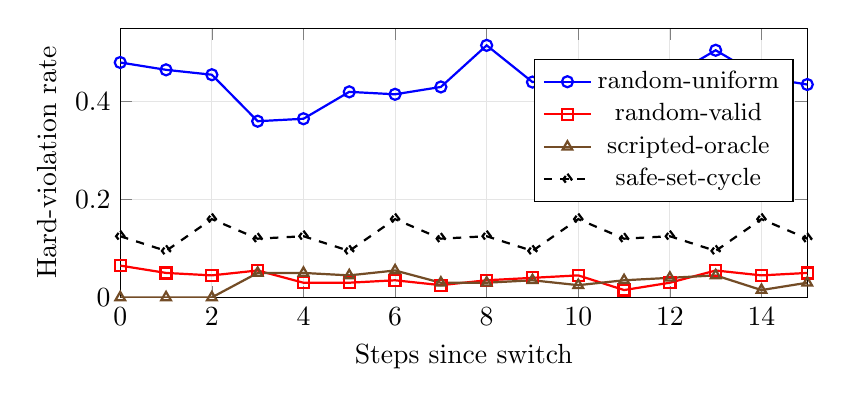
\begin{tikzpicture}
\begin{axis}[width=0.85\linewidth,height=5cm,xlabel={Steps since switch},ylabel={Hard-violation rate},
  ymin=0,ymax=0.55,xmin=0,xmax=15,legend style={font=\small,at={(0.98,0.62)},anchor=east},grid=major,grid style={gray!20}]
\addplot+[mark=o,thick] coordinates {(0,0.48)(1,0.465)(2,0.455)(3,0.36)(4,0.365)(5,0.42)(6,0.415)(7,0.43)(8,0.515)(9,0.44)(10,0.455)(11,0.445)(12,0.45)(13,0.505)(14,0.45)(15,0.435)};
\addplot+[mark=square,thick] coordinates {(0,0.065)(1,0.05)(2,0.045)(3,0.055)(4,0.03)(5,0.03)(6,0.035)(7,0.025)(8,0.035)(9,0.04)(10,0.045)(11,0.015)(12,0.03)(13,0.055)(14,0.045)(15,0.05)};
\addplot+[mark=triangle,thick] coordinates {(0,0)(1,0)(2,0)(3,0.05)(4,0.05)(5,0.045)(6,0.055)(7,0.03)(8,0.03)(9,0.035)(10,0.025)(11,0.035)(12,0.04)(13,0.045)(14,0.015)(15,0.03)};
\addplot+[mark=diamond,thick,dashed] coordinates {(0,0.125)(1,0.095)(2,0.16)(3,0.12)(4,0.125)(5,0.095)(6,0.16)(7,0.12)(8,0.125)(9,0.095)(10,0.16)(11,0.12)(12,0.125)(13,0.095)(14,0.16)(15,0.12)};
\legend{random-uniform,random-valid,scripted-oracle,safe-set-cycle}
\end{axis}
\end{tikzpicture}
\caption{Post-switch hard-rule violation rate under the corrected reward (200 episodes per policy). \todo{add grpo-\hidden{} / \dial{} / \oracle{} curves.}}
\label{fig:decay}
\end{figure}

\subsection{Trained policies}
\label{sec:trained}

\todo{This subsection is intentionally empty. Every adapter trained before the audit in \S\ref{sec:audit} (one 300-step \hidden{} run and one 50-step pilot) was trained on prompts in which 12 of the 24 pitches were rendered one semitone flat. Those adapters are therefore not reported as results. Required before this section can be written: base-zeroshot and grpo-\{\oracle,\dial,\hidden\} retrained on the corrected pipeline, evaluated with \texttt{eval/evaluate\_llm.py} on the fixed set, with action validity, the full Table~\ref{tab:baselines} metrics, the paired comparisons of grpo-\hidden{} vs.\ random-valid and vs.\ safe-set-cycle, and the arm contrasts \hidden{} vs.\ \dial{} vs.\ \oracle{} across seeds.}

The pre-registered expectation is scripted-oracle $>$ grpo-\oracle{} $>$ grpo-\dial{} $\geq$ grpo-\hidden{} $\geq$ random-valid. The protocol states in advance that grpo-\hidden{} failing to exceed random-valid is a reportable outcome, not a failed experiment. A second failure mode must be checked explicitly even under the corrected reward: convergence toward the safe set, signalled by safe-set occupancy approaching 1 with adaptation success near 0.

\section{Validity Audit}
\label{sec:audit}

Table~\ref{tab:audit} lists every defect found during development that affected a reported or reportable quantity. Defects marked $\ast$ were found in a final audit of the whole pipeline, carried out before any trained policy was evaluated on the fixed set. Each defect now has a regression test. We report them because the first two would have invalidated the central comparison without any visible symptom.

\begin{table}[t]
\centering\small
\caption{Defects found and fixed. ``Affected'' lists what each defect would have corrupted.}
\label{tab:audit}
\begin{tabular}{@{}p{0.43\linewidth}p{0.5\linewidth}@{}}
\toprule
Defect & Affected \\
\midrule
$\ast$ Prompt decoded note pitches with truncation (\texttt{int}) from float32 $n/23$, so 12 of 24 pitches rendered a semitone flat (e.g.\ \sw{Sa} shown as lower-octave \sw{Ni}, \sw{Re} as \sw{re}). & Every LLM prompt in training and evaluation; all prior adapters. \\
$\ast$ Note-history slots were left-aligned, so in the first 3 steps the last-listed note was an empty slot, not the note just played. & Early-episode prompts ($\approx$5\% of training rows). \\
Default ``no call'' value \texttt{[0,0,0,0]} was truthy, so the call-response reward fired on every training step against a call never shown to the model; the call phrase was also never rendered in the prompt. & First training run's reward signal and task. \\
$\ast$ A partner call was flagged on the terminal step, where it can never be answered. & Echo rate and coherence understated by a factor of $7/8$. \\
$\ast$ The pre-registered adherence metric counts only forbidden swaras, not out-of-scale ones. & Post-switch errors such as Ma$^\sharp$ carried into Bhairav; random-uniform reads 0.875 instead of 0.559. Amended (\S\ref{sec:protocol}). \\
Adaptation-bonus phrase matching compared tuples to lists and could never succeed. & Adaptation bonus was never paid. \\
$\ast$ Result fingerprints omitted the environment, drift, and prompt modules. & A stale LLM result would have passed the staleness check. \\
$\ast$ Leap penalty uncapped (to $-3.2$), violating the bounded-penalty invariant. & Reward ranked the degenerate safe-set policy above raga-informed play (\S\ref{sec:baselines}). \\
$\ast$ Ascending rule judged on the 3-note contour, not the move into the note. & Legal descents into Pa penalised; some rising Ga$\to$Pa unpenalised. \\
$\ast$ Training's Monte-Carlo continuation dropped the episode's remaining switch and partner calls. & Training returns near a switch or call. \\
$\ast$ Smaller fixes: empty history slots rendered as fake notes; all-Sa call rendered as ``no call''; linear call tension; \texttt{reset()} kept the previous episode's dial; 16-bit evaluation of 4-bit-trained adapters; unvalidated \texttt{/call} input; blocking \texttt{/infer}. & Prompts, call reward, evaluation fidelity, demo server. \\
\bottomrule
\end{tabular}
\end{table}

The metric amendments are additive. The pre-registered metrics are unchanged and reported alongside the amended ones. The reward changes alter the environment itself, so every baseline was regenerated. All amendments were made before any trained policy was scored.

\section{Related Work}
\label{sec:related}

\paragraph{Contextual and hidden-parameter MDPs; non-stationarity.} Contextual MDPs condition the reward and dynamics on an observed context~\citep{hallak2015cmdp}. Hidden-parameter MDPs make that parameter latent and inferred from interaction~\citep{doshivelez2013hipmdp}. Our three arms ablate exactly this axis while holding the dynamics fixed. Work on non-stationary RL addresses drifting or switching environments through change or context detection~\citep{dasilva2006context,padakandla2020survey}. Our setting is a single abrupt switch within one short episode, judged on within-episode recovery.

\paragraph{Meta-RL and in-context RL.} RL$^2$~\citep{duan2016rl2} and learning-to-learn~\citep{wang2016learning} train recurrent policies that adapt within an episode through their hidden state. Algorithm Distillation~\citep{laskin2022ad} and Decision-Pretrained Transformers~\citep{lee2023dpt} obtain in-context RL from sequence models pretrained across many tasks. \citet{krishnamurthy2024explore} find that off-the-shelf LLMs explore poorly in context without substantial intervention. \env{} asks a narrower question: whether a small instruction-tuned LLM, fine-tuned with GRPO on one task family, uses reward feedback written into its prompt to detect a regime switch.

\paragraph{RL for music.} Sequence Tutor~\citep{jaques2017sequencetutor} fine-tunes a melody model with RL against music-theory rewards under a KL constraint. RaveForce~\citep{lan2019raveforce} offers an RL environment for audio-level music generation. Computational work on Hindustani music has focused on recognition: raga identification from pitch-class statistics~\citep{chordia2007raag} and motif spotting from audio~\citep{ross2012motifs}. We generate under symbolic raga constraints, add mid-episode rule drift, and add a call-response partner. To our knowledge, no prior environment combines these.

\paragraph{Reward hacking.} \citet{skalse2022rewardhacking} formalise when optimising a proxy reward can reduce the true objective. The safe-set result in \S\ref{sec:baselines} is a concrete instance, caught by calibration baselines before any optimisation, where the proxy ranked a non-adapting policy above an informed one.

\section{Limitations}
\label{sec:limits}

\begin{itemize}[leftmargin=*,itemsep=2pt]
  \item \textbf{No trained-model results yet.} The central question, whether grpo-\hidden{} performs in-context regime inference, is unanswered (\S\ref{sec:trained}).
  \item \textbf{Residual reward risk.} The corrected reward ranks the scripted baselines as intended, but a learned policy may find exploits that no scripted baseline probes. The contour-contrast term in particular pays every policy, call-blind or not.
  \item \textbf{Reward amended after pre-registration.} The leap floor and the move-based direction rule were changed after the protocol was written, before any trained policy was evaluated. Results under the original reward are reported for comparison (Table~\ref{tab:paired}).
  \item \textbf{Simplified musicology.} Two ragas, two octaves, discrete pitches, no ornaments. Bhairav's defining oscillation (\sw{andolan}) on re and dha cannot be represented, so its \sw{pakad}s are discrete approximations. The \sw{vadi}/\sw{samvadi} assignments follow the encoded source and are not universal across traditions.
  \item \textbf{Implicit raga signal in \hidden{}.} Raga-legal partner calls leak information about the active raga in every arm, so \hidden{} isolates the absence of an explicit identifier, not of all information.
  \item \textbf{Monte-Carlo continuation.} Training returns use a random reference policy over 8 steps, so they score an action under the reference policy's future behaviour, not the learner's.
  \item \textbf{Scale.} One 0.5B model family, single-GPU budgets, and few seeds limit statistical power for arm contrasts.
\end{itemize}

\section{Broader Impact and Ethics}
The environment uses Hindustani raga grammar as a formal rule system. It does not claim to model musical quality or to substitute for musicians, and rule adherence is not musicality. Human-facing audio in the companion demo uses third-party samples under CC BY 3.0 and CC0 licences, attributed in the repository. No human-subject data was collected. A listening study is outside the scope of this draft.

\section{Reproducibility Statement}
Code, the raga rule definitions, the evaluation-set generator, the metric implementations, the baseline result files, and the statistics script are in the accompanying repository under the MIT licence. Every result file embeds a fingerprint: the git SHA plus content hashes of the training requirements, the raga rules, the reward, both environment classes, the drift manager, the prompt renderer, the evaluation-set generator, the metrics, the baseline policies, the LLM policy wrapper, the rollout harness, and the evaluation runner. A result whose fingerprint does not match the current tree is treated as stale. Baselines need no GPU and are regenerated with \texttt{python -m eval.evaluate --all}; the statistics with \texttt{python -m paper.scripts.baseline\_stats}. Training runs on a free Colab T4 notebook. The environment is also served over HTTP with an OpenEnv-style manifest~\citep{openenv} for the interactive demo; no reported number goes through the HTTP path.

\section*{LLM Usage Disclosure}
An AI coding assistant was used to write and review parts of the codebase, to run the pipeline audit in \S\ref{sec:audit}, and to draft this manuscript. All bibliography entries were retrieved from bibliographic APIs (arXiv, CrossRef, Semantic Scholar, OpenAlex) rather than generated. Entries the APIs could not fully resolve are marked for human verification. \todo{author to confirm and edit this statement to the venue's policy.}

\bibliographystyle{plainnat}
\bibliography{refs}

\appendix

\section{Full Reward Specification}
\label{app:reward}
\begin{table}[h]
\centering\small
\begin{tabular}{@{}llr@{}}
\toprule
Layer & Term (condition) & Value \\
\midrule
1 Hard & forbidden swara & $-2.0\cdot g$ \\
 & ascending-rule violation (move into note is upward; swara legal but not ascending-allowed) & $-1.0\cdot g$ \\
 & out-of-scale swara & $-1.5\cdot g$ \\
 & \multicolumn{2}{l}{\footnotesize $g=0.2$ during the 3-step grace period after a switch, else 1. First matching rule returns; layers 2--4 skipped.} \\
2 Soft & legal note & $+0.2$ \\
 & \sw{vadi} / \sw{samvadi} & $+0.4$ / $+0.3$ \\
 & \sw{vadi} drought $D_v>8$ & $\max(-0.05(D_v-8),\,-1.0)$ \\
 & leap $|\Delta n|>7$ & $\max(-0.2(|\Delta n|-7),\,-1.0)$ \\
 & same swara as each of previous 3 notes & $-0.3$ \\
 & \sw{vadi} with duration index $\ge 2$ & $+0.15$ \\
3 Sequence & \sw{pakad} completed (last $\le 6$ notes, first match in list order) & $+1.0\times$multiplier \\
 & \sw{pakad} drought $D_p>12$ & $\max(-0.03(D_p-12),\,-0.5)$ \\
 & \sw{vadi} on \sw{sam} / weak note on \sw{sam} & $+0.8$ / $-0.4$ \\
 & \sw{vadi} or \sw{samvadi} on strong beat $\{0,4,12\}$ & $+0.2$ \\
4 Call & tension $>0.5$ and \sw{vadi} & $+0.5\cdot$tension \\
 & move direction $\neq$ neutral and $\neq$ call contour & $+0.3$ \\
 & swara equals call's last swara (once per call) & $+0.4$ \\
5 Drift & new-raga \sw{pakad} within 5 steps of switch (once) & $+3.0$ \\
\bottomrule
\end{tabular}
\end{table}
Call contour is ascending if the call's last swara exceeds its first, and descending otherwise (ties count as descending). Droughts count steps since the \sw{vadi} was last played, or since a \sw{pakad} was last completed.

\section{Prompt Format}
\label{app:prompt}
Exact output of the rendering function for the \hidden{} arm at episode start, immediately after a switch to Bhairav. The previous-step outcome line is supplied for illustration; at a true episode start it is absent. Only the one note actually in the history is listed; empty slots are omitted. \dial{} inserts \texttt{Raga dial: 0.75} before the tala line. \oracle{} inserts \texttt{Active raga: bhairav (dial=0.75 GRACE PERIOD - rules just changed)} and \texttt{Steps since last rule change: 0.0 (normalised)}.
\begin{verbatim}
<|system|>
You are an expert Indian classical musician composing in a raga. Given
the current musical context, choose the next note action (0-95). Action
encodes: note (0-23, absolute pitch across two registers) +
duration_index (0-3) * 24. Output ONLY the integer, nothing else.
<|user|>
Tala position: beat 0/16
Recent notes (oldest first): Sa(quarter)
Partner's call phrase: none yet
Human call tension: 0.00 (how unresolved their phrase was)
Pakad drought: 0.00 (0=just played a phrase, 1=very long since last phrase)
Vadi drought: 0.00 (0=vadi just played, 1=long since)
Last action: Ma(sixteenth) -> outcome: penalised (-2.00)
Choose action (0-95):
<|assistant|>
\end{verbatim}
(Lower-octave notes are rendered with the prefix \b{n}, i.e.\ n with a macron below, e.g.\ \b{n}Ni.)

\section{Provenance of Reported Numbers}
\label{app:provenance}
Table~\ref{tab:baselines}: \texttt{eval/results/\{random-uniform,random-valid,safe-set-cycle,scripted-oracle\}.json}. Tables~\ref{tab:paired}--\ref{tab:decomp} and Figure~\ref{fig:decay}: \texttt{paper/data/baseline\_stats.json}, produced by \texttt{paper/scripts/baseline\_stats.py} (bootstrap seed 0). Table~\ref{tab:decomp}'s component sums come from the same rollouts. All files were regenerated on 2026-10-07 after the audit fixes. Each embeds content hashes of every file its numbers depend on; these, not the git SHA, are the staleness check, since a result committed with its code necessarily records the parent commit (with a dirty-tree flag). Original-reward figures in Table~\ref{tab:paired} come from the same scripts run at the pre-fix commit \texttt{919ae82}.

\section{Paper Checklist (NeurIPS-style, abridged)}
\begin{enumerate}[leftmargin=*,itemsep=1pt]
  \item Claims match results: yes. No trained-model claim is made.
  \item Limitations: \S\ref{sec:limits}.
  \item Theory: none claimed.
  \item Reproducibility: \S\ref{sec:training}, \S\ref{sec:protocol}, appendices; open TODOs on TRL defaults and seeds.
  \item Code and data: yes (repository).
  \item Experimental details: \S\ref{sec:training}--\ref{sec:protocol}.
  \item Statistical significance: paired-bootstrap CIs, Wilcoxon tests, $d_z$ (Table~\ref{tab:paired}).
  \item Compute: Colab T4; \todo{GPU-hours per run from training logs}.
  \item Ethics: no human subjects; licensed audio only in the demo.
  \item Broader impacts: \S\ref{sec:limits} and the impact section.
  \item Safeguards: not applicable (no high-risk release).
  \item Licences: MIT (code); CC BY 3.0 and CC0 (demo audio); Qwen2.5 \todo{state model licence}.
  \item New assets: environment and evaluation set, documented in the repository.
  \item Human subjects / IRB: not applicable.
  \item LLM usage: disclosed above.
\end{enumerate}

\end{document}
